% Opening > Navier--Stokes
\section{Navier--Stokes}

% [1 min] Collage of the announcement and its reception.
\begin{frame}{September 8, 2026: Math changes forever}
  \centering
  \begin{tikzpicture}[x=1cm, y=1cm]
    % bounding box = visible extent of the collage, so it centres on the page
    \useasboundingbox (0.48,0) rectangle (14.25,-6.25);
    \def\img{images/announcement_images}
    % the result: blow-up visualization (background made transparent; original in \img)
    \node at (2.9,-3.1) {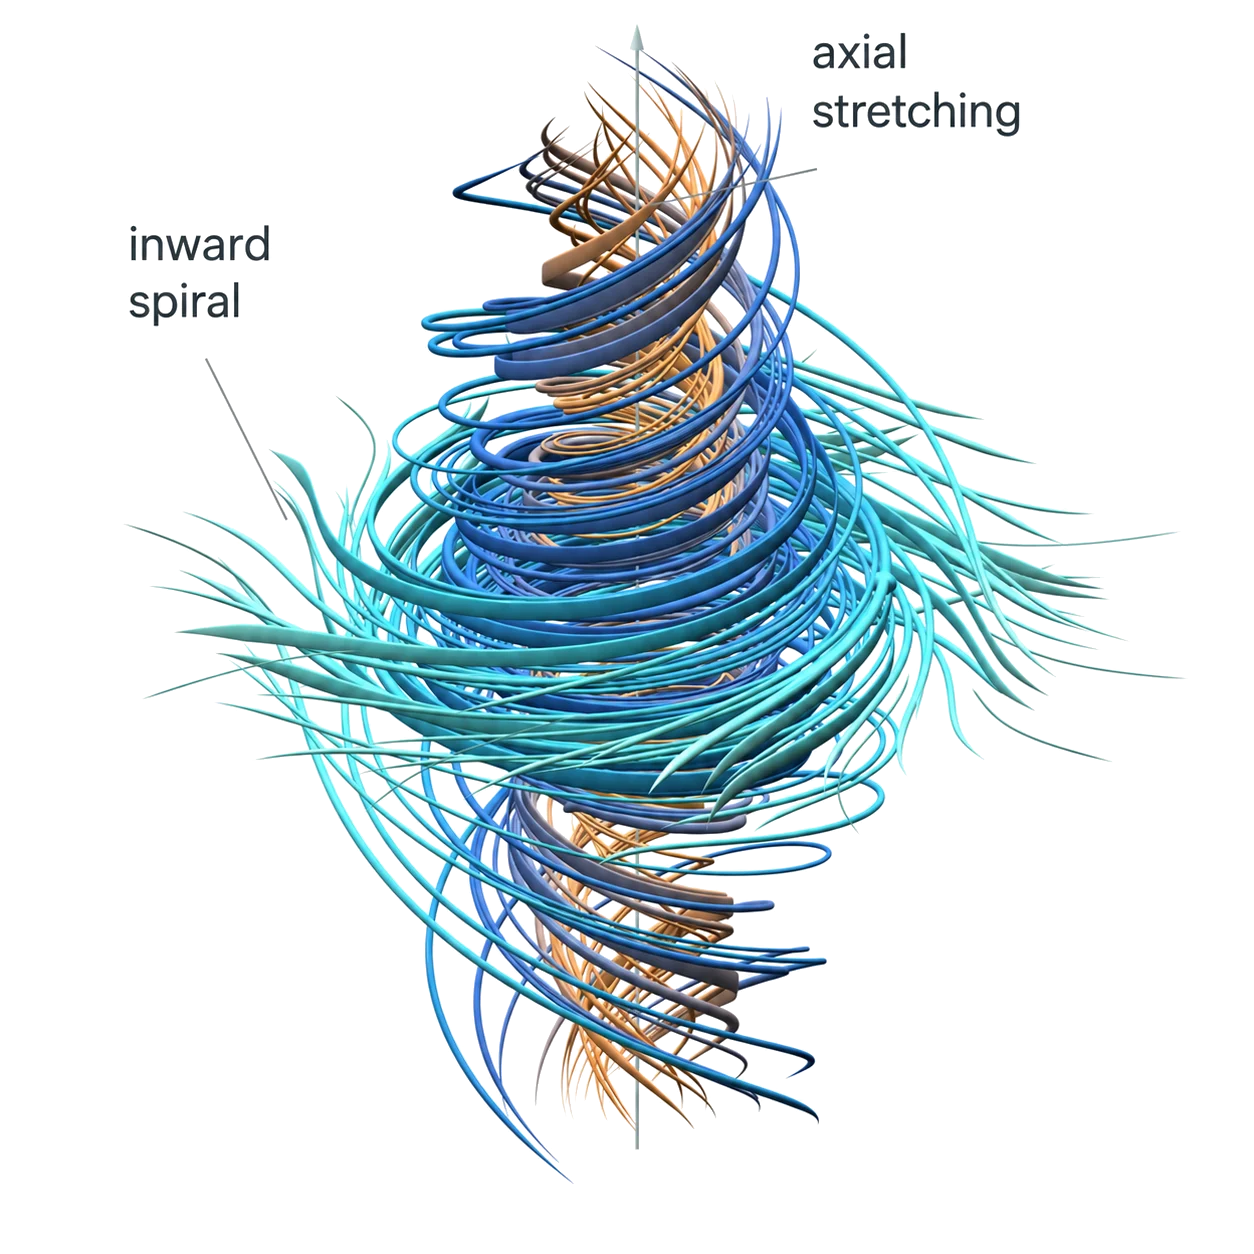
\includegraphics[height=6.1cm]{images/blowup_transparent.png}}; % openai.com/index/navier-stokes-solution/
    % press coverage
    \node[collagecard, rotate=2]    at (8.15,-3.55) {\includegraphics[width=4.9cm]{\img/nature_openai.png}};
    \node[collagecard, rotate=-2.5] at (12.0,-2.95) {\includegraphics[width=4.3cm]{\img/tech_desk_openai.png}};
    \node[collagecard, rotate=1.5]  at (11.2,-5.35) {\includegraphics[width=5.0cm]{\img/forbes_announcement.png}};
    % the announcement itself, on top
    \node[collagecard, rotate=-1]   at (9.6,-0.95)  {\includegraphics[width=7.4cm]{\img/openai_ns_announce.png}};
    % the mood
    \node[collagecard, rotate=-4]   at (6.1,-5.1)   {\includegraphics[width=2.3cm]{\img/cat_discover.png}}; % x.com/MozeTech/status/2097383226503532611
  \end{tikzpicture}
  \slidesources{Sources: OpenAI on X, 8 Sep 2026 \textbullet{} Nature news, 8 Sep 2026 \textbullet{} Technology Desk, 9 Sep 2026 \textbullet{} Forbes \textbullet{} Visualization: OpenAI \textbullet{} Meme: @MozeTech on X}
\end{frame}

% [2 min] The usual route vs OpenAI's route. Builds in three steps:
% (1) the usual route, (2) OpenAI's route skipping peer review, (3) the Lean
% proof sitting in peer review's column, and the takeaway.
\begin{frame}{Why believe it?}
  \centering
  \begin{tikzpicture}[x=1cm, y=1cm, font=\sffamily\footnotesize]
    % bounding box = visible extent of the diagram, so it centres on the page
    \useasboundingbox (0.68,0.1) rectangle (14.01,-6.2);
    % column positions
    \def\ca{2.9}\def\cb{5.4}\def\cc{7.9}\def\cd{10.4}\def\ce{12.9}
    % column headers
    \foreach \x/\t in {\ca/Discovery, \cb/Write-up, \cc/Verification, \cd/Dissemination, \ce/Acceptance}
      \node[colhead] at (\x,-0.15) {\t};

    % ---- (1) the usual route -------------------------------------------------
    \node[lane=black!70] at (1.75,-1.05) {The usual\\route};
    \node[stage] (a1) at (\ca,-1.05) {Human proof};
    \node[stage] (a2) at (\cb,-1.05) {Preprint\\[-1pt]{\scriptsize arXiv}};
    \node[stage] (a3) at (\cc,-1.05) {Peer review\\[-1pt]{\scriptsize referees}};
    \node[stage] (a4) at (\cd,-1.05) {Journal\\[-1pt]{\scriptsize publication}};
    \node[stage] (a5) at (\ce,-1.05) {Accepted\\[-1pt]{\scriptsize Clay: +2 years}};
    \foreach \u/\v in {a1/a2, a2/a3, a3/a4, a4/a5} \draw[flow] (\u) -- (\v);
    \draw[span] (\ca-1.1,-1.85) -- node[note, below=1pt] {months to years} (\ce+1.1,-1.85);

    % ---- (2) OpenAI's route ---------------------------------------------------
    \onslide<2->{
      \node[lane=PennBlue] at (1.75,-3.05) {OpenAI\\Sep 2026};
      \node[stage=PennBlue] (b1) at (\ca,-3.05) {10,000 agents\\[-1pt]{\scriptsize 88 hours}};
      \node[stage=PennBlue] (b2) at (\cb,-3.05) {AI-written\\paper};
      \node[stage, draw=black!35, dashed, fill=white, text=black!40] (b3) at (\cc,-3.05)
        {Peer review\\[-1pt]{\scriptsize skipped}};
      \node[stage=PennBlue] (b4) at (\cd,-3.05) {Announced\\[-1pt]{\scriptsize on X, 8 Sep}};
      \node[stage=PennBlue] (b5) at (\ce,-3.05) {Taken\\seriously};
      \draw[flow=PennBlue] (b1) -- (b2);
      \draw[flow=PennBlue] (b4) -- (b5);
    }
    \only<2>{
      % bypass arc under the skipped box (where the Lean proof appears next)
      \draw[flow=PennBlue] (b2.south east) to[out=-35, in=-145] (b4.south west);
    }

    % ---- (3) what stood in for peer review -----------------------------------
    \onslide<3->{
      \node[stage=PennRed, line width=0.9pt] (b3l) at (\cc,-4.45)
        {\textbf{Lean proof}\\[-1pt]{\scriptsize kernel-checked, +17 h}};
      \draw[flow=PennBlue] (b2.south) |- (b3l.west);
      \draw[flow=PennBlue] (b3l.east) -| (b4.south);
      \draw[span] (\ca-1.1,-5.25) -- node[note, below=1pt] {88 + 17 hours of compute} (\ce+1.1,-5.25);
    }
  \end{tikzpicture}
  \slidesources{Sources: OpenAI, 8 Sep 2026 \textbullet{} Reisinger et al., \emph{The Mathematical Sciences in an AI-enabled World}, AcadMathSci, Oct 2026 \textbullet{} Clay Mathematics Institute, Millennium Prize rules}
\end{frame}

